
\chapter {Device handling}

The functions in a haptics device class can be divided into two classes:

\begin{itemize}
\item Device handling routines.
\item Routines for determining what and how should be rendered haptically
for the device. 
\end{itemize}

The device handling routines are functions for initializing the
device, reading positions and sending forces. 

The other functions are for setting the haptics rendering algorithm
to use and set the geometries and force effects that are to be
rendered.

\section{Calibration}
By default the coordinates given by the haptics device classes are
given in millimetres in the local coordinate space of the haptics
device. Often this is not the coordinate system a user wants
though, and therefore HAPI provides a mean to change the coordinate
system by adding a calibration matrix. The position given by the
getPosition() function will then be pos = matrix * orig\_pos. It is
also possible to calibrate the orientation and the result will be in
the same way, i.e. orn = orn\_calib * orig\_orn. In this case the
calibration value will not be a matrix, but a Rotation object.

\section{Layering}
When adding shapes to be rendered at the haptics device, one can
specify what ``layer'' in which it should be rendered. Each layer have
its own haptics rendering algorithm, which makes it possible to render
different shapes with different haptics rendering algorithms on one
haptics device. The resulting force will be the sum of the forces from
each layer. A common use is, for example in medical simulation, to
specify shapes for different tissue layers in different haptic
layers. For example, if rendering a hand, one might use one layer for
the skin and one layer for the bone of the hand. This will make it
possible to feel the hard bone through the soft skin. If the shapes
were specified in only one layer, the user would feel only the skin
geometry, since the proxy stays on the surface. Specifying the bone in
a second layer will add a new separate proxy for all the shapes in
that layer. 

\begin{figure} 
  \centering 
  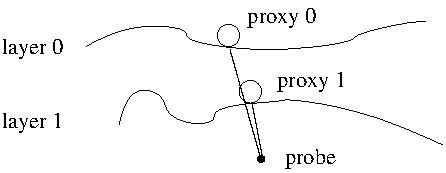
\includegraphics{images/layering.pdf}
  \caption{To the left all surface are part of layer 0. The proxy is then stopped at the first surface and the
underlying surface will never be felt. To the right the two surfaces are put in two different layers which
each has its own proxy, which means it will be felt.} 
  \label{Layering_fig} 
\end{figure}

If no haptics rendering algorithm is specified for a layer, no forces
will be generated from that layer.
 
By default all operations use layer 0.

\section{The HAPIHapticsDevice abstract base class}
The HAPIHapticsDevice abstract base class is the base class for all
haptics device implementations. It contains the functions that are
available for all haptics devices.  

\subsection{Device handling functions}

Most common device handling functions:

\begin{itemize}
\item ErrorCode initDevice() -  Does all the initialization needed for the
device before starting to use it.
\item ErrorCode releaseDevice() - Releases all resources that were allocated
in initDevice.
\item ErrorCode enableDevice() - Enabling the device means that the
positions and forces will be updated.  
\item ErrorCode disableDevice() - Stop the forces and position
from being updated, but does not release the device.
\item DeviceValues getDeviceValues() - Get a structure with all the
  device values that are recorded each frame (such as position,
  velocity,etc)
\item Vec3 getPosition() - Get the position of the haptics device (in
  mm)
\item Vec3 getVelocity() - Get the velocity of the haptics device (in
  mm/s)
\item Rotation getOrientation() - Get the orientation of the haptics
  device stylus (if 6 DOF input).
\item bool getButtonStatus( unsigned int button\_nr ) - get the status
  for a given button on the haptics device.
\end{itemize}

The error code returned is HAPI::HAPIHapticsDevice::SUCCESS on success.

\subsection{Calibration functions}
\begin{itemize}
\item void setPositionCalibration( const Matrix4 \&m ) - Set the
 position calibration matrix
\item const Matrix4 \&getPositionCalibration() - Get the current
 position calibration matrix
\item void setOrientationCalibration( const Rotation \&r ) - Set the
  orientation calibration
\item const Rotation \&getOrientationCalibration() - Get the
  current orientation calibration
\end{itemize}


\subsection{Haptics rendering functions}
Following are the most commonly used functions for changing what and
how to render objects with the haptics device. 

\begin{itemize} 

\item void setHapticsRenderer( HAPIHapticsRenderer *r, unsigned int
  layer = 0 ) - Set the haptics rendering algoritm to use for a
  specific layer on the haptics device

\item void addShape( HAPIHapticShape *shape, unsigned int layer = 0 )
  - Render a shape on the given layer. The shape will be rendered
  until removed.
\item void removeShape( HAPIHapticShape *shape, unsigned int layer = 0
  ) - Remove a shape currently being rendered.
\item void clearShapes( unsigned int layer = 0 ) - Remove all shapes
  on a layer. 

\item void addEffect( HapticForceEffect *effect ) - Add a haptic
  effect to render by the haptics device. The effect will be rendered
  until removed.
\item void removeEffect( HapticForceEffect *effect ) - Remove a haptic
  effect currently being rendered.
\item void clearEffects() - Remove all haptic effects currently rendered.
\end{itemize}

The above functions works at a temporary local copy of effects and
shapes. The haptics is rendered in a different loop and in order to
transfer the changes made to that loop the user has to call the
transferObjects() function. It is made in this way so only one
synchronization call is needed between the two threads, instead of one
for each call to the functions above.

Example:

{
\tt
{\hlstd }{\hlline \ \ \ \ 1\ }{\hlslc // make changes to the objects you want to render}\leavevmode\par
{\hlline \ \ \ \ 2\ }{\hlstd hd}{\hlsym $\mathord{-}$$\mathord{>}$}{\hlstd }{\hlkwd clearEffects}{\hlstd }{\hlsym ();}\leavevmode\par
{\hlline \ \ \ \ 3\ }{\hlstd hd}{\hlsym $\mathord{-}$$\mathord{>}$}{\hlstd }{\hlkwd addEffect}{\hlstd }{\hlsym ( }{\hlstd }{\hlkwa new }{\hlstd HapticForceField }{\hlsym );}\leavevmode\par
{\hlline \ \ \ \ 4\ }{\hlstd hd}{\hlsym $\mathord{-}$$\mathord{>}$}{\hlstd }{\hlkwd addEffect}{\hlstd }{\hlsym ( }{\hlstd }{\hlkwa new }{\hlstd HapticSpring }{\hlsym );}\leavevmode\par
{\hlline \ \ \ \ 5\ }{\hlstd }\leavevmode\par
{\hlline \ \ \ \ 6\ }{\hlslc // nothing has changed on what is rendered yet, call transferObjects}\leavevmode\par
{\hlline \ \ \ \ 7\ }{\hlstd }{\hlslc // to transfer the changes to the haptics rendering thread.}\leavevmode\par
{\hlline \ \ \ \ 8\ }{\hlstd hd}{\hlsym $\mathord{-}$$\mathord{>}$}{\hlstd }{\hlkwd transferObjects}{\hlstd }{\hlsym ();}{\hlstd }\leavevmode\par
}


See the doxygen documentation for a full listing of the functions
available. 

\section{Example}
Following is an example on a simple program that initialize a haptics
device and sends a constant force of 1 N in the positive x-direction.

{
\tt
{\hlstd }{\hlline \ \ \ \ 1\ }\leavevmode\par
{\hlline \ \ \ \ 2\ }{\hldir \#include $\mathord{<}$AnyHapticsDevice.h$\mathord{>}$}\leavevmode\par
{\hlline \ \ \ \ 3\ }{\hlstd }{\hldir \#include $\mathord{<}$HapticForceField.h$\mathord{>}$}\leavevmode\par
{\hlline \ \ \ \ 4\ }{\hlstd }\leavevmode\par
{\hlline \ \ \ \ 5\ }{\hlkwa using namespace }{\hlstd HAPI}{\hlsym ;}\leavevmode\par
{\hlline \ \ \ \ 6\ }{\hlstd }\leavevmode\par
{\hlline \ \ \ \ 7\ }{\hlkwb int }{\hlstd }{\hlkwd main}{\hlstd }{\hlsym (}{\hlstd }{\hlkwb int }{\hlstd argc}{\hlsym , }{\hlstd }{\hlkwb char}{\hlstd }{\hlsym * }{\hlstd argv}{\hlsym []) $\{$}\leavevmode\par
{\hlline \ \ \ \ 8\ }{\hlstd }{\hlstd\ \ }{\hlstd }{\hlslc // The force to render}\leavevmode\par
{\hlline \ \ \ \ 9\ }{\hlstd }{\hlstd\ \ }{\hlstd Vec3 force\_{}to\_{}render }{\hlsym $\mathord{=}$ }{\hlstd }{\hlkwd Vec3}{\hlstd }{\hlsym ( }{\hlstd }{\hlnum 1}{\hlstd }{\hlsym , }{\hlstd }{\hlnum 0}{\hlstd }{\hlsym , }{\hlstd }{\hlnum 0 }{\hlstd }{\hlsym );}\leavevmode\par
{\hlline \ \ \ 10\ }{\hlstd \leavevmode\par
{\hlline \ \ \ 11\ }}{\hlstd\ \ }{\hlstd }{\hlslc // Create a new haptics device, using any device connected.}\leavevmode\par
{\hlline \ \ \ 12\ }{\hlstd }{\hlstd\ \ }{\hlstd auto\_{}ptr}{\hlsym $\mathord{<}$ }{\hlstd AnyHapticsDevice }{\hlsym $\mathord{>}$ }{\hlstd }{\hlkwd device}{\hlstd }{\hlsym ( }{\hlstd }{\hlkwa new }{\hlstd AnyHapticsDevice }{\hlsym );}\leavevmode\par
{\hlline \ \ \ 13\ }{\hlstd \leavevmode\par
{\hlline \ \ \ 14\ }}{\hlstd\ \ }{\hlstd }{\hlslc // initialize the device}\leavevmode\par
{\hlline \ \ \ 15\ }{\hlstd }{\hlstd\ \ }{\hlstd }{\hlkwa if}{\hlstd }{\hlsym ( }{\hlstd device}{\hlsym $\mathord{-}$$\mathord{>}$}{\hlstd }{\hlkwd initDevice}{\hlstd }{\hlsym () !$\mathord{=}$ }{\hlstd HAPIHapticsDevice}{\hlsym ::}{\hlstd SUCCESS }{\hlsym ) $\{$}\leavevmode\par
{\hlline \ \ \ 16\ }{\hlstd }{\hlstd\ \ \ \ }{\hlstd }{\hlslc // initilization failed, print error message and quit}\leavevmode\par
{\hlline \ \ \ 17\ }{\hlstd }{\hlstd\ \ \ \ }{\hlstd cerr }{\hlsym $\mathord{<}$$\mathord{<}$ }{\hlstd device}{\hlsym $\mathord{-}$$\mathord{>}$}{\hlstd }{\hlkwd getLastErrorMsg}{\hlstd }{\hlsym () $\mathord{<}$$\mathord{<}$ }{\hlstd endl}{\hlsym ;}\leavevmode\par
{\hlline \ \ \ 18\ }{\hlstd }{\hlstd\ \ \ \ }{\hlstd }{\hlkwa return }{\hlstd }{\hlnum 1}{\hlstd }{\hlsym ;}\leavevmode\par
{\hlline \ \ \ 19\ }{\hlstd }{\hlstd\ \ }{\hlstd }{\hlsym $\}$}\leavevmode\par
{\hlline \ \ \ 20\ }{\hlstd \leavevmode\par
{\hlline \ \ \ 21\ }}{\hlstd\ \ }{\hlstd }{\hlslc // enable the device(forces and positions will be updated)}\leavevmode\par
{\hlline \ \ \ 22\ }{\hlstd }{\hlstd\ \ }{\hlstd device}{\hlsym $\mathord{-}$$\mathord{>}$}{\hlstd }{\hlkwd enableDevice}{\hlstd }{\hlsym ();}\leavevmode\par
{\hlline \ \ \ 23\ }{\hlstd \leavevmode\par
{\hlline \ \ \ 24\ }}{\hlstd\ \ }{\hlstd }{\hlslc // add the force effect to render}\leavevmode\par
{\hlline \ \ \ 25\ }{\hlstd }{\hlstd\ \ }{\hlstd device}{\hlsym $\mathord{-}$$\mathord{>}$}{\hlstd }{\hlkwd addEffect}{\hlstd }{\hlsym ( }{\hlstd }{\hlkwa new }{\hlstd }{\hlkwd HapticForceField}{\hlstd }{\hlsym ( }{\hlstd force\_{}to\_{}render }{\hlsym ) );}\leavevmode\par
{\hlline \ \ \ 26\ }{\hlstd \leavevmode\par
{\hlline \ \ \ 27\ }}{\hlstd\ \ }{\hlstd }{\hlslc // transfer the effect to the haptics loop.}\leavevmode\par
{\hlline \ \ \ 28\ }{\hlstd }{\hlstd\ \ }{\hlstd device}{\hlsym $\mathord{-}$$\mathord{>}$}{\hlstd }{\hlkwd transferObjects}{\hlstd }{\hlsym ();}\leavevmode\par
{\hlline \ \ \ 29\ }{\hlstd \leavevmode\par
{\hlline \ \ \ 30\ }}{\hlstd\ \ }{\hlstd }{\hlslc // wait for keyboard press, then finish program}\leavevmode\par
{\hlline \ \ \ 31\ }{\hlstd }{\hlstd\ \ }{\hlstd }{\hlkwa while}{\hlstd }{\hlsym (}{\hlstd }{\hlkwa true}{\hlstd }{\hlsym ) $\{$}\leavevmode\par
{\hlline \ \ \ 32\ }{\hlstd \leavevmode\par
{\hlline \ \ \ 33\ }}{\hlstd\ \ }{\hlstd }{\hlsym $\}$}\leavevmode\par
{\hlline \ \ \ 34\ }{\hlstd \leavevmode\par
{\hlline \ \ \ 35\ }}{\hlstd\ \ }{\hlstd }{\hlkwa return }{\hlstd }{\hlnum 0}{\hlstd }{\hlsym ;}\leavevmode\par
{\hlline \ \ \ 36\ }{\hlstd }{\hlsym $\}$}{\hlstd }\leavevmode\par
}
 

\section{Supported haptics devices}
The haptics devices currently supported by HAPI are:

\begin{itemize}
\item PHANToM Devices from SensAble Technologies (implemented in the
  PhantomHapticsDevice class)
\item Delta and Omega devices from ForceDimension(implemented in the
  ForceDimensionHapticsDevice class)
\item 2 DOF Pantograph and something else (TODO) from Quanser.
 (implemented in the QuanserHapticsDevice class). This feature is not yet fully
 tested and should be considered prototype.
\item Falcon from Novint (implemented in the FalconHapticsDevice class ). 
This feature is not yet fully tested and should be considered prototype.
\end{itemize}

Also there is the AnyHapticsDevice class which uses any supported
device connected to the computer.

\subsection{Adding support for new devices}
\label{ssAddingHapticsSupport}

Support for new devices can easily be added to HAPI by subclassing the
HAPIHapticsDevice class and implement the abstract functions. The
functions to implement are:

\begin{itemize}
\item bool initHapticsDevice() - initialize the haptics device. Return
  true on success, otherwise false and set an error message. 
\item bool releaseHapticsDevice() - releases all resources held by the
  haptics device. Return true on success, otherwise false and set an
  error message. 
\item void updateDeviceValues( DeviceValues \&dv, HAPITime dt ) - fill
  in the DeviceValues structures with the current values from the
  haptics device(values are e.g. position, velocity, etc). dt is the
  time in seconds since the last update.
\item void sendOutput( DeviceOutput \&dv, HAPITime dt ) - render the
  output given in the DeviceOutput structure (such as force and torque)
  on the haptics device. dt is the time in seconds since the last update.
\end{itemize}

Look at the PhantomHapticsDevice and ForceDimensionHapticsDevice classes for
example implementations. 

Also in order for your new device to be recognised by the
AnyHapticsDevice class, you will have to register the haptics device
to a database of available devices. This is done by adding the a
static member in your new class:

In header file:

{
\tt
{\hlstd }{\hlline \ \ \ \ 1\ }{\hlkwb static }{\hlstd HapticsDeviceRegistration device\_{}registration}{\hlsym ;}{\hlstd }\leavevmode\par
}


In .cpp file:

{
\tt
{\hlstd {\hlline \ \ \ \ 1\ }HAPIHapticsDevice}{\hlsym ::}{\hlstd HapticsDeviceRegistration\leavevmode\par
{\hlline \ \ \ \ 2\ }MyNewHapticsDevice}{\hlsym ::}{\hlstd device$\backslash$\_{}registration}{\hlsym (}\leavevmode\par
{\hlline \ \ \ \ 3\ }{\hlstd }{\hlstd\ \ \ \ \ \ \ \ \ \ \ \ \ \ \ \ \ \ \ \ \ \ \ \ \ \ \ \ }{\hlstd }{\hlstr "MyDevice"}{\hlstd }{\hlsym ,}\leavevmode\par
{\hlline \ \ \ \ 4\ }{\hlstd }{\hlstd\ \ \ \ \ \ \ \ \ \ \ \ \ \ \ \ \ \ \ \ \ \ \ \ \ \ \ \ }{\hlstd $\backslash$\&}{\hlsym (}{\hlstd newInstance}{\hlsym $\mathord{<}$ }{\hlstd MyNewHapticsDevice }{\hlsym $\mathord{>}$)}\leavevmode\par
{\hlline \ \ \ \ 5\ }{\hlstd }{\hlstd\ \ \ \ \ \ \ \ \ \ \ \ \ \ \ \ \ \ \ \ \ \ \ \ \ \ \ \ }{\hlstd }{\hlsym );}{\hlstd }\leavevmode\par
}


The string given as first argument is the name of your new device.

